\documentclass[12pt,a4paper]{scrartcl}
\usepackage[ngerman, english]{babel}
\usepackage[T1]{fontenc}
\usepackage[utf8]{inputenc}
\usepackage[color=yellow!15]{todonotes}
\usepackage{graphicx}
\usepackage[numbers, square]{natbib}

% used for line numbering
%\usepackage{lineno}

% The following parameters seem to provide a reasonable page setup.
\topmargin 0.0cm
\oddsidemargin 0.2cm
\textwidth 16cm 
\textheight 21cm
\footskip 1.0cm


%The next command sets up an environment for the abstract to your paper.
\newenvironment{sciabstract}{%
\begin{quote} \bfseries}
{\end{quote}}


% If your reference list includes text notes as well as references,
% include the following line; otherwise, comment it out.

\renewcommand\refname{References and Notes}

% The following lines set up an environment for the last note in the
% reference list, which commonly includes acknowledgments of funding,
% help, etc.  It's intended for users of BibTeX or the {thebibliography}
% environment.  Users who are hand-coding their references at the end
% using a list environment such as {enumerate} can simply add another
% item at the end, and it will be numbered automatically.

\newcounter{lastnote}
\newenvironment{scilastnote}{%
\setcounter{lastnote}{\value{enumiv}}%
\addtocounter{lastnote}{+1}%
\begin{list}%
{\arabic{lastnote}.}
{\setlength{\leftmargin}{.22in}}
{\setlength{\labelsep}{.5em}}}
{\end{list}}


% Include your paper's title here

\title{\textbf{ \Large{Decentralized, autonomous sensor fault detection using neural networks}} }


\author
{Katrin Jahr, Robert Schlich$^{1}$\\
\\
\normalsize{$^{1}$Degree program “Civil Engineering” (M.Sc.)}\\
\normalsize{Bauhaus-Universität Weimar, Germany}\\
\\
\normalsize{katrin.jahr@uni-weimar.de}\\
\normalsize{robert.schlich@uni-weimar.de}
}


% Include the date command, but leave its argument blank.
\date{}



%%%%%%%%%%%%%%%%% END OF PREAMBLE %%%%%%%%%%%%%%%%



\begin{document} 

% Double-space the manuscript.

\baselineskip32pt

% Make the title.

\maketitle 



% Place your abstract within the special {sciabstract} environment.

\begin{sciabstract}

The dependability and the accuracy of structural health monitoring systems are significantly affected by sensor faults. 
In this paper, the design and implementation of a wireless structural health monitoring system, capable of decentralized autonomous fault detection, are presented. 
For self-detecting sensor faults, each sensor node predicts its expected sensor data and compares it to the measured sensor data. 
The predictions are computed using neural networks \textbf{with measured sensor data} of adjacent sensor nodes.
In laboratory experiments, devised to validate the proposed approach, several simulated sensor faults are detected.
These results indicate that the use of neural networks increases the dependability and the accuracy of structural health monitoring systems.

\end{sciabstract}

%----------------------------------------------------------------------------------------

%\linenumbers % Schaltet Zeilennummerierung ein
%\modulolinenumbers[5] % nur jede 5. Zeile
\section*{Dictionary}

\begin{tabular}{|l|l|}
\hline 
Sensorknoten (SunSPOT) & sensor node \\ 
\hline 
einzelner Messsensor (Thermometer) & sensor \\ 
\hline 
Knoten im neuronalen Netz & neuron \\ 
\hline 
eine abgeschlossene Messungreihe & test run \\ 
\hline 
gemessene Werte & sensor data \\ 
\hline 
vorhergesagte Werte & predicted data \\ 
\hline 
durch Vorhersage erwartete Werte & expected data \\ 
\hline 
einzelner Messwert & measurement \\ 
\hline 
Test & laboratory experiments\\ 
\hline
tatsächliche, nicht virtuelle Messung & actual measurement \\
\hline
Messaufbau & test setup \\
\hline

\end{tabular} 

%----------------------------------------------------------------------------------------

\section*{Introduction}

Civil engineering structures are exposed to external impacts over several decades. 
To ensure the structural stability and evaluate the conditions of civil engineering structures, structural health monitoring (SHM) systems can be installed.
\cite[4]{BisbySHM} defines SHM as "a non-destructive \textit{in-situ} structural evaluation method that uses any of several sensors which are attached to, or embedded in, a structure". 
The obtained sensor data is "collected, analyzed and stored" over long periods of time.
Analysis of the sensor data can reveal abnormal changes in material and geometric behaviour early on.

Traditionally, the sensor nodes are wired with cables and connected to computer systems.
However, using wired SHM systems has several disadvantages, including expensive wiring, high personnal costs and inaccessibility of optimal positions with wiresIn this case.
In wireless SHM systems, the sensor nodes communicate with a base station via radio, ruling out wiring-specific problems.
When using wireless SHM systems, one has to consider battery life and sensor node \textit{sychronization}.
\todo{wird später darauf eingegangen? Sonst raus.}

Over time, sensors can break and become faulty. Failures can either occur suddenly, or be due to gradual loss of accuracy.
To ensure the dependability and the accuracy of the SHM system, these sensor faults must be detected and isolated in real time. 
A simple approach to fault detection is the installation of physically redundant sensors.
Faulty sensors can easily be identified through the deviation of their measurements from the measurements of other sensors.
Physical redundancy, although efficient at sensor fault detection, has the disadvantage of increased installation and maintenance costs. 
A technologically more advanced approach, called analytical redundancy, applies knowledge of the structure and the SHM system itself to compute virtual sensor measurements for each sensor. 
For example, a FEM model could be used in combination with data from adjacent sensor nodes to calculate a virtual measurement of one sensor.
If analytical redundancy is implemented correctly, virtual measurements always simulate a correct working sensor; therefore actual measurements deviating from their virtual counterparts indicate faulty sensors.\citep{Smarsly2014}

In this study, analytical redundancy is realized by artificial neural networks.
Artificial neural networks consist of interconnected data processing elements called neurons. 
Neurons are grouped in different layers; they consist of one input layer, a number of hidden layers and one output layer.
Artificial neural networks have the distinct ability of learning by adjusting the weights of the inter-neuron connections, until a set of given input variables results in the desired output variables.
If implemented correctly, a neural network can be trained to approximate any mathematical functions with arbitrary accuracy \citep{Li2011}.

This paper is organized as follows:
First, a wireless structural health monitoring system is designed and implemented. 
Next, a neural network is implemented in each sensor node and trained to predict the measurements of said node in order to detect faults. 
The system is then tested in laboratory experiments. 
Finally, the experimental results are analyzed and future research directions proposed.

%----------------------------------------------------------------------------------------

\newpage

\section*{Design and implementation of the wireless structural health monitoring system}
In the following section, a brief descriptions of SHM systems general is given. Furthermore, the used wireless SHM system is introduced and the Java implementation is described.

According to \cite[5]{BisbySHM}, a structural health monitoring system commonly consists of the following components:
1. data acquisition,
2. data transmission, 
3. data processing,
4. data storage,
5. diagnostics and 
6. information retrieval.

Tasks 1 to 3 are usually implemented on site, while tasks 4 to 6 are usually implemented on computer systems off site.
A wireless SHM system installed on the building site consists of sensor nodes attached to the construction, a base station, and a local computer. 
The base station, which can be an external device or a computer program, links the individual sensor nodes with each other and the local computer.
To each sensor node, several sensors measuring different physical quantities may be connected. 
In this project, the acceleration is measured using wireless sensor nodes and a basestation of the type "Oracle Sun SPOT". 
The 3-axis digital output accelerometer with sensitivity ranging between $ \pm $ 2G and $\pm$ 8G has a maximum sample rate of 125Hz. \cite[9]{eDemo2010}

In operation, the sensor nodes acquire sensor data and may perform initial processing.
The processed data is then transmitted via radio to the local computer, where it is stored for analysis and diagnosis.
In this project, the data is transmitted from the sensor nodes to the basestation by radio, and from the basestation to the local computer via USB cable.
On the computer, the data is stored in a MySQL database.

\todo[inline]{vielleicht eine Abbildung? SunSPOTs? Aufbau SHM?}


\textbf{3. paragraph: UML / Java implementaion}

%According to [3], a structural health monitoring system basically consists of the following components:
%1. data acquisition, 2. data communication, 3. data processing, 4. data storage, 5. diagnostics and 6. data retrieval.
%
%
%
%For autonomous fault detection in wireless SHM systems, an integrated fault detection and synchronization strategy is implemented into a wireless SHM system. The SHM system consists of wireless sensor nodes and a base station. The sensor nodes are installed on the monitored structure and the base station links the wireless SHM system and a local computer.
%
%
%In the present study, wireless sensor nodes of the type “Oracle Sun SPOTs” are used. The sensor nodes are Java-programmable enabling embedded analyses and the sensor nodes include a 3-dimensional accelerometer, temperature and other sensors (Oracle Lab, 2014). In this study, acceleration measurements taken from the structure are used for analyzing the structural condition. Furthermore, the radios of the sensor nodes ensure wireless communications between the sensor nodes as well as between the sensor nodes and the base station in order to transmit monitoring data or control commands. The base station is able to receive monitoring data measured by the sensor nodes, and the base station can store the data in a database installed on the local computer. The main Java classes are shown in an Unified Modelling Language diagram (UML diagram), which is a standard way to visualize the implementation of a application. The following UML diagrams (cp. Figure 1 and Figure 2) show just the main classes embedded into the base station and the sensor nodes. In the following subsection, the implementation of the main components of the fault detection strategy, including synchronization and fault detection, are shown.

\newpage

%----------------------------------------------------------------------------------------

\section*{Implementation and training of neural networks}

Neural networks are implemented into the sensor nodes using SNIPE\footnote{}, a open source Java Library.
\begin{figure}[ht]
    \centering
    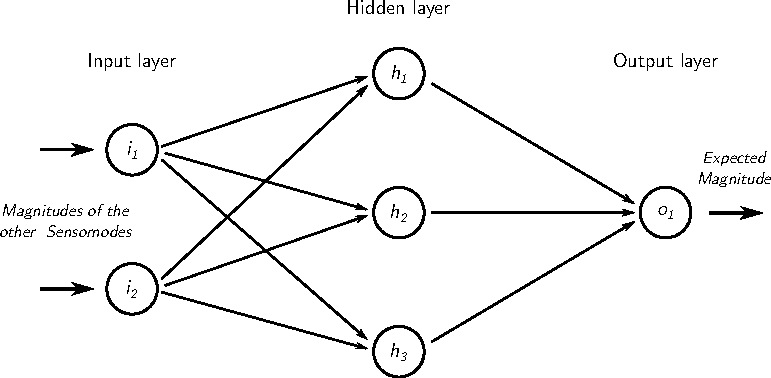
\includegraphics{figures/neuralnetwork.pdf}
    \caption{Schematic drawing of an artificial neural network with three layers}
    \label{fig:neuralnetwork}
\end{figure}
\todo[inline]{Grafik kann nacher noch an unser neuronales Netz angepasst werden}


%\begin{itemize}
%\item neurons
%\item layer
%\item weights
%\item activation function / identity function
%\end{itemize}

\textbf{2. paragraph: proposed nn}

\begin{itemize}
\item SNIPE? implementation in java?
\item activation function / identity function
\end{itemize}

\textbf{3. paragraph: learning general}

\begin{itemize}
\item set with test values
\item iterative weight adjustment
\end{itemize}

\textbf{4. paragraph?: learning, proposed}

%----------------------------------------------------------------------------------------


\newpage
\section*{Laboratory experiments}

%\begin{itemize}
%\item test structure
%\item sensor installation
%\item type of excitation, acceleration is measured
%\end{itemize}

To validate the proposed approach, the SHM system was installed on a test structure in order to conduct laboratory experiments.
The test structure consists of four metal sheets with an area of 20~cm by 60~cm and 4~mm of thickness.
Those metal sheets are mounted on threaded rods with a vertical clearance of approximately 40~cm.
At the bottom, the threaded rods are fixed into a block of solid wood with an area of 40~cm by 60~cm and a height of 50~cm.
The SHM system is installed onto the test structure by strapping a SunSPOT to each of the metal sheets.
The finished laboratory setup is shown in figure~\ref{fig:teststructure}.
\todo{Bild ersetzen durch ein Bild mit den fertig installierten SPOTS}
The structure is excited by pulling one of the metal sheets a few centimeters to the side and releasing it.
This method of excitation ensures, that the structure vibrates in its Eigenfrequency with little interferences.

\begin{figure}[h!]
    \centering
    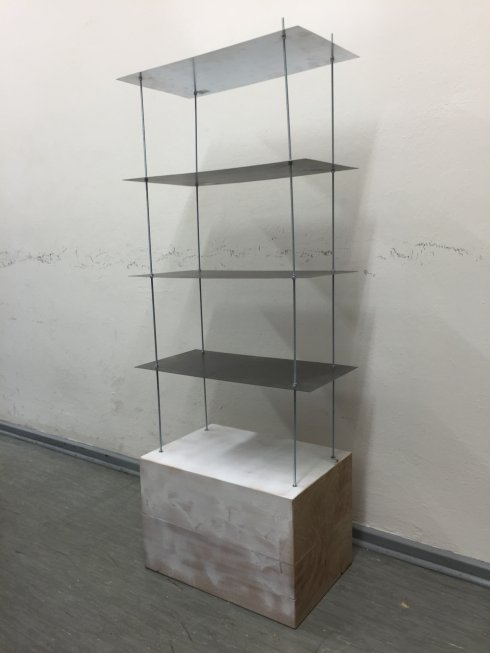
\includegraphics[scale=0.3]{figures/teststructure.jpg}
    \caption{Picture of the laboratory setup}
    \label{fig:teststructure}
\end{figure}


\textbf{2. paragraph: data measurement and processing}

\begin{itemize}
\item learning phase
\item excitation
\item sensors start measuring
\item sensor nodes \textbf{perform fft} - what is fft
\item sensor nodes exchange frequencies
\item neural networks check integrity
\item if no faults detected, sensor nodes send data to base station
\end{itemize}

\textbf{3. paragraph: sensor fault detection}

\begin{itemize}
\item simulation of sensor fault
\item neural networks check integrity -> error!
\item sensor node sends alert to base station
\end{itemize}

%----------------------------------------------------------------------------------------

%\section*{Discussion of the experimental results}

%----------------------------------------------------------------------------------------

\section*{Summary and conclusions}

Everything went better than expected!
%----------------------------------------------------------------------------------------

\bibliographystyle{unsrtnat}
\bibliography{literature}

\end{document}
